\chapter{User Interface}

\section{Main Window}
In the Main Window you can see the following editors and views (see \ref{main}):
\begin{itemize}
	\item Architecture Editor
	\item Role View
	\item Workflow View
	\item Minimap
\end{itemize}

\begin{figure}[h!]
\begin{center}
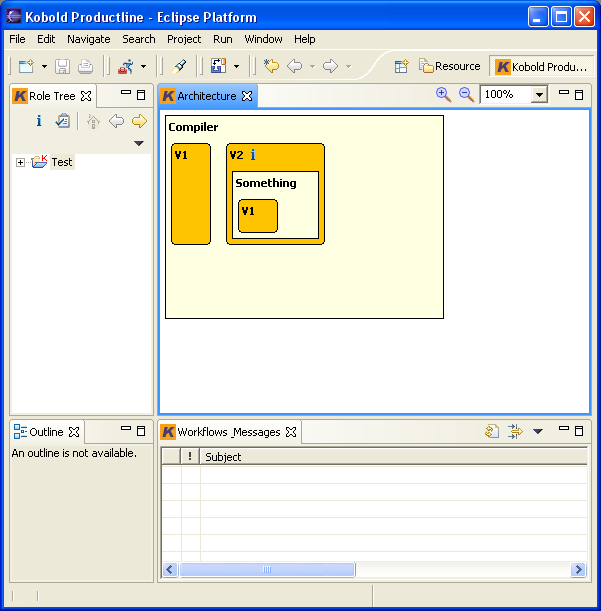
\includegraphics[width=15cm]{main.png}
   \caption{Main Window}
\label{main}
\end{center}
\end{figure}\par

The menu offers you in addition to the Eclipse standard options the following
possibilities:
\begin{itemize}
	\item Checking out a product
	\item Changing Kobold properties
\end{itemize}
Look up the explanations in the "Tutorial" section.

\section{Architecture Editor}

The Architecture Editor (see \ref{architecture}) displays the architecture of the product,
or product line respectively, that is selected in the Role View. \par

\begin{figure}[h!]
\begin{center}

\includegraphics[width=15cm]{architecture.png}
   \caption{Architecture Editor}
\label{architecture}
\end{center}
\end{figure}\par

Architectures are directed graphs that consist of nodes and edges. 
Nodes represent components, variants and releases. Directed edges represent
any relationship between nodes.\par

The Architecture Editor offers you the following options:
\begin{itemize}
%	\item Creating a Core Asset
	\item Creating a variant
	\item Creating a component
	\item Creating a release
	\item Creating a meta node
	\item Deleting a component, variant or release
	\item Deleting a meta node
	\item Creating a dependency edge
	\item Creating an exclusion edge
	\item Deleting an edge
	\item Marking a component, variant or release "deprecated"
	\item Setting the maintainers of a component
	\item Selecting resources for variants and releases
	\item Moving an item
	\item Changing the size of an item
%	\item Filtering the Architecture View
%	\item Creating a custom component
%	\item Deleting a custom component
	\item Composing a product
	\item Export
\end{itemize}

Most of them can be reached through the palette (see \ref{palette}), that opens up when you click on it.

\begin{figure}[h!]
\begin{center}

\includegraphics[width=4cm]{palette.png}
   \caption{The palette}
\label{palette}
\end{center}
\end{figure}\par

Please look up the explanations in the "Tutorial" section.

\section{Role View}

The Role View shows the current projects that are checked out in your workspace 
(see \ref{roletree}).
A project is usually a product line. You can navigate between the 
different projects by selecting them. If you open the tree, you see the name
of the product line. Double-click on 'Architecture' and the Architecture Editor will open. The open tree also 
displays all products, PLEs and core assets that belong to the productline.

\begin{figure}[h!]
\begin{center}

\includegraphics[width=7cm]{roletree.png}
   \caption{Role View}
\label{roletree}
\end{center}
\end{figure}\par

When you right-click on a project, a context menu will open where you can choose 
between different actions (see \ref{rolekontext}). Among those are:

\begin{itemize}
%	\item Renaming a product
%	\item Changing a product
%	\item Setting a product on deprecated
%	\item Setting a module on deprecated
	\item Creating a user
	\item Deleting a user
	\item Change one's password
	\item Update full name
	\item Configure asset
	\item Suggesting an asset for a Core Group
	\item Generate a metainfo document
	\item Export
%	\item Changing a user role
\end{itemize}
Look up the explanations in the "Tutorial" section.

\begin{figure}[h!]
\begin{center}

\includegraphics[width=5cm]{rolekontext.png}
   \caption{Role Tree Context Menu}
\label{rolekontext}
\end{center}
\end{figure}\par



\section{Workflow View}

In the bottom of the window you can see the Workflow View which displays all 
the messages and workflows for the current user (see \ref{workflow}). 

\begin{figure}[h!]
\begin{center}

\includegraphics[width=15cm]{workflow.png}
   \caption{Workflow/Task View}
\label{workflow}
\end{center}
\end{figure}\par

Double-click on an entry and a 
separate dialog will be opened where you can read the details of that message or
workflow (see \ref{workflowdialog}).

\begin{figure}[h!]
\begin{center}

\includegraphics[width=5cm]{workflowdialog.png}
   \caption{Message Dialog}
\label{workflowdialog}
\end{center}
\end{figure}\par

When you right-click on a message, a context menu will open where you can choose 
between different actions (see \ref{workflowkontext}). Among these are:

\begin{itemize}
	\item Fetching messages
	\item Deleting the selected message
%	\item Filtering sent messages
\end{itemize}
Look up the explanations in the "Tutorial" section.

\begin{figure}[h!]
\begin{center}

\includegraphics[width=7cm]{workflowkontext.png}
   \caption{Message Context Menu}
\label{workflowkontext}
\end{center}
\end{figure}\par

The Workflow View offers you the following additional options:
\begin{itemize}
	\item Writing a mail
	\item Answering a mail
	\item Suggesting an asset for a Core Group
	\item Dealing with a Core Group suggestion
\end{itemize}
Look up the explanations in the "Tutorial" section.

\section{Minimap}

The Minimap (see \ref{map}) is on the left side beneath the Role View. It shows the whole architecture.
By clicking at one spot on the map, the Architecture Editor automatically centers on that
spot. 

\begin{figure}[h!]
\begin{center}

\includegraphics[width=10cm]{outline.png}
   \caption{Minimap}
\label{map}
\end{center}
\end{figure}\par


\section{Server Administration Tool (SAT)}

The Server Administration Tool provides you with an interface to your server. \par
During the starting process you have to enter the URL and password of the server 
you want to administrate. Once the tool is started, you have the following 
possibilities:

\begin{itemize}
	\item create a product line
	\item delete a product line
	\item upgrade an existing user to PLE status
	\item remove PLE rights
	\item get a list of all existing commands
	\item create a new user
	\item delete a user
	\item get a list of all productlines
	\item get a list of all PLEs of a productline
	\item get a list of all users
	\item exit the tool
\end{itemize}

